\documentclass{homework}

\title{Estudo Dirigido 1 - ALA}
\author{Carlos Henrique Bravo Serrado\\ 119136241}

\pgfplotsset{compat=1.17}
\begin{document}

\maketitle

\exercise
(a) Sejam $u$ e $v$ os vetores normais das retas $2x + 3y = 0$ e $x - 2y = 0$, respectivamente. Podemos reescrever $2x + 3y = 0$ como $\langle (x,y)|(2,3)\rangle = 0$, então, u = $(2,3)$, pois se o produto interno der 0, é normal. Podemos aplicar a mesma lógica para encontrar $v=(1,-2)$.

Para encontrar o ângulo formado basta calcular o produto interno $\langle u|v\rangle$. \par
\[\langle u|v\rangle = \norm{u}\norm{v}cos(\theta)\]
\[\langle u|v\rangle = u_1 v_1 + u_2 v_2\]
\[\norm{u}\norm{v}cos(\theta) = u_1 v_1 + u_2 v_2\]

\[cos(\theta) = \frac{u_1 v_1 + u_2 v_2}{\norm{u}\norm{v}}\]
Substituindo as variáveis com os valores respectivos e sendo $\norm{u} = \sqrt{u_1^2 + u_2^2}$ e $\norm{v} = \sqrt{v_1^2 + v_2^2}$.
\[cos(\theta) = \frac{(2)(1) + (3)(-2)}{\sqrt{13}\sqrt{5}} = \frac{-4}{\sqrt{65}}\]
\[\theta = arccos(\frac{-4}{\sqrt{65}})\]
(b)

\begin{center}
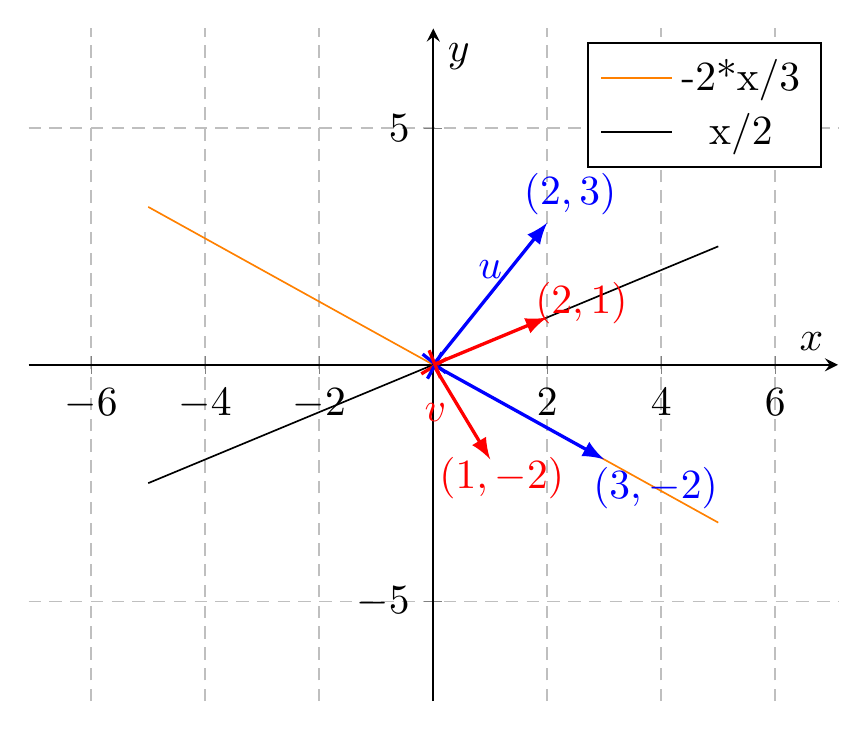
\begin{tikzpicture}[>=latex, scale=1.5]
    \begin{axis}[
axis lines=middle,
grid,
grid style={densely dashed},
xlabel=\(x\), ylabel=\(y\),
xmin=-7.1, xmax=7.1,
ymin=-7.1, ymax=7.1
                ]
    \addplot [no markers, orange]{-2*x/3};
    \addlegendentry{-2*x/3};
    \addplot [no markers, black]{x/2};
    \addlegendentry{x/2};
    \addplot [|->, thick,  blue] coordinates {(0,0) (2,3)} node[midway, above] {$u$} node[pos=1.2] {$(2,3)$};
    \addplot [|->, thick,  red] coordinates {(0,0) (1,-2)} node[midway, left] {$v$} node[pos=1.2] {$(1,-2)$};
    \addplot [|->, thick,  blue] coordinates {(0,0) (3,-2)} node[pos=1.3] {$(3,-2)$};
    \addplot [|->, thick,  red] coordinates {(0,0) (2,1)} node[pos=1.3] {$(2,1)$};

    \end{axis}
\end{tikzpicture}
\end{center}

\exercise*
Queremos provar que $det(U) = \pm1$ para a matriz U dada.
\[U_\beta =
\begin{bmatrix}
u_{11} & u_{12}\\ 
u_{21} & u_{22}
\end{bmatrix}
\]
\[det(U_\beta) = u_{11}u_{22} - u_{12}u_{21} = \langle (u_{11},u_{12})|(u_{22},-u_{21})\rangle\]
O vetor $(u_{22},-u_{21})$ é um vetor normal a $u_2$ e, portanto, é paralelo a $u_1$. O ângulo formado entre $u_1$ e $u_2^\perp$ pode ser $0$ ou $\pi$.
\[det(U_\beta) = \langle (u_{11},u_{12})|(u_{22},-u_{21})\rangle = \langle u_1|u_2^\perp\rangle = \norm{u_1}\norm{u_2^\perp}cos(\theta)\]
Como os vetores $u_1$ e $u_2^\perp$ são unitários, sua norma é 1. Portanto, $det(U_\beta) = cos(\theta)$. Como $\theta$ pode ser $0$ ou $\pi$, $cos(\theta)$ pode ser $1$ ou $-1$. \par
Com isso, $det(U_\beta) = \pm1$. $\blacksquare$

\exercise*
(a) Para ser ortonormal, o segundo vetor precisa ser ortogonal e normal. Um vetor ortogonal a $(u_{11},u_{12})$ é $u_2 = (u_{12},-u_{11})$. A norma de ambos vetores é $1$, então são normais ($\frac{\sqrt{(\pm2)^2 + (\pm1)^2}}{\sqrt{5}} = \frac{\sqrt{5}}{\sqrt{5}} = 1$). Falta apenas definir o sentido de $u_2$. 

Para ser orientado positivamente, $det(U_\beta) = 1$. O determinante desta base é $-u_{11}^2 - u_{12}^2$. Como os quadrados são sempre positivos, a soma de dois números negativos será negativo, então $det(U_\beta) = -1$. Basta trocar o sinal, definindo $u_2 = (-u_{12},u_{11})$, isto é, $u_2 = \frac{1}{\sqrt{5}}(-2,-1)$.

(b) As coordenadas do ponto $p = (-2,6)$ 
em relação a base $\beta$ é $(Proj_{u_1}(p),Proj_{u_2}(p))$.
\[Proj_{u_1} = \langle p|u_1\rangle\cdot u_1 = \frac{(-2)(-1) + (6)(2)}{\sqrt{5}} \cdot u_1 = \frac{14}{\sqrt{5}} \cdot u_1\]
\[Proj_{u_2} = \langle p|u_2\rangle\cdot u_2 = \frac{(-2)(-2) + (6)(-1)}{\sqrt{5}} \cdot u_2 = \frac{-2}{\sqrt{5}} \cdot u_2\]
Então na base $\beta$, as coordenadas do ponto $p$ são $\frac{1}{\sqrt{5}}(14,-2)$.

\exercise*
Para encontrar o operador que leva dos vértices finais ao iniciais, é possível usar o fato que as bases canônicas $(1,0)$ e $(0,1)$ fazem parte dos pontos. 
\[T^{-1}(e_1) = (2,3)\]
\[T^{-1}(e_2) = (-6,4)\]
\[(T^{-1})_\epsilon = 
\begin{bmatrix}
2 & -6\\
3 & 4
\end{bmatrix}\]
\[\]
\[(T)_\epsilon = \frac{1}{det((T^{-1})_\epsilon)}
\begin{bmatrix}
4 & 6\\
-3 & 2
\end{bmatrix} = \frac{1}{26}
\begin{bmatrix}
4 & 6\\
-3 & 2
\end{bmatrix}\]

\exercise*
Para realizar uma rotação e depois uma reflexão, basta fazer a multiplicação dos operadores correspondentes. Primeiro encontrando a matriz responsável por realizar uma rotação.
\[(\rho_{\pi/3})_\epsilon = 
\begin{bmatrix}
cos(\pi/3) & -sen(\pi/3)\\
sen(\pi/3) & cos(\pi/3)
\end{bmatrix} = \frac{1}{2}
\begin{bmatrix}
1 & -\sqrt{3}\\
\sqrt{3} & 1
\end{bmatrix}\]
Agora para a reflexão, precisa encontrar um vetor unitário diretriz da reta. Como a reta é $y = 2x$, podemos reescrever como $2x - y = 0$, de onde tira-se o vetor $u = (2,-1)$. Normalizando o vetor, tem-se que $u = \frac{1}{\sqrt{5}}(2,-1)$.
\[(R)_\epsilon = \begin{bmatrix}
1 & 0\\
0 & 1
\end{bmatrix} - \frac{2}{5}
\begin{bmatrix}
2\\
-1
\end{bmatrix}
\begin{bmatrix}
2 & -1
\end{bmatrix} = 
\begin{bmatrix}
1 & 0\\
0 & 1
\end{bmatrix} - \frac{2}{5}
\begin{bmatrix}
4 & -2\\
-2 & 1
\end{bmatrix} = \frac{1}{5}
\begin{bmatrix}
-3 & 4\\
4 & 3
\end{bmatrix}\]
\[(T)_\epsilon = R\rho = \frac{1}{10}
\begin{bmatrix}
-3 & 4\\
4 & 3
\end{bmatrix}
\begin{bmatrix}
1 & -\sqrt{3}\\
\sqrt{3} & 1
\end{bmatrix} = \frac{1}{10}
\begin{bmatrix}
4\sqrt{3} - 3 & 4 + 3\sqrt{3}\\
4 + 3\sqrt{3} & 3 - 4\sqrt{3}
\end{bmatrix}\]
(b) Se o determinante de um operador linear for $\pm1$, ele será uma rotação ou reflexão dependendo do sinal.
\[det(T) = \frac{(4\sqrt{3}-3)(3-4\sqrt{3}) - (4+3\sqrt{3})(4+3\sqrt{3})}{100} = \frac{-100}{100} = -1\]
Como o determinante é -1, $(T)_\epsilon$ é uma reflexão.

\exercise
Para ser uma reflexão, o determinante dessa matriz precisa ser -1.
\[det(Q) = \frac{b}{3} - a^2 = -1\]
\[b = 3a^2 - 3\]
Para encontrar os valores de $b$, precisamos primeiro encontrar os valores de $a$, então vamos encontrar os espelhos primeiro. Para isso, basta encontrar os vetores diretores.
\[Q = I - 2nn^\top\]
\[\begin{bmatrix}
n_1^2 & n_1n_2\\
n_1n_2 & n_2^2
\end{bmatrix} = \frac{1}{2}
\left(\begin{bmatrix}
1 & 0\\
0 & 1
\end{bmatrix} - 
\begin{bmatrix}
\frac{1}{3} & a\\
a & 3a^2 - 3
\end{bmatrix}\right) =
\begin{bmatrix}
\frac{1}{3} & \frac{-a}{2}\\
\frac{-a}{2} & \frac{4 - 3a^2}{2}
\end{bmatrix}\]
\begin{center}
\[
\begin{cases}
n_1^2 = \frac{1}{3}\\
n_1 n_2 = -\frac{a}{2}\\
n_2^2 = \frac{4-3a^2}{2}
\end{cases}
\]
\end{center}
\[n_1 = \frac{1}{\sqrt{3}}\]
\[n_2 = -\frac{a}{2n_1} = -\frac{a\sqrt{3}}{2}\]
\[n_2^2 = \frac{4-3a^2}{2} = \frac{3a^2}{4} \Longrightarrow a = \pm\frac{2\sqrt{2}}{3}\]
\[n_2 = \pm\frac{2\sqrt{2}}{3}\frac{\sqrt{3}}{2} = \pm\frac{\sqrt{2}}{\sqrt{3}}\]

Os valores das variáveis serão $a = \pm\frac{2\sqrt{2}}{3}$ e $b = -\frac{1}{3}$. Os espelhos serão as retas formadas pelos vetores diretores $(\frac{1}{\sqrt{3}},\frac{\sqrt{2}}{\sqrt{3}})$ e $(\frac{1}{\sqrt{3}},-\frac{\sqrt{2}}{\sqrt{3}})$, pois $n_2$ tem 2 valores possíveis.

\exercise*
Se a base $\beta$ é ortonormal, seus vetores formam um ângulo de $\frac{\pi}{2}$ entre si. Utilizando o caso base no qual $u_1 = (1,0)$, $u_2$ possui 2 valores possíveis: $(0,1)$ e $(0,-1)$. Analisando cada caso:

Para a prova da ida, vamos provar a contra-positiva. "Se não existe uma rotação anti-horária, a base não é positivamente orientada". Se $u_2 = (0,-1)$, nenhuma rotação leva $e_2$ até $u_2$ enquanto mantém $u_1$ fixo em $e_1$, pois qualquer que seja o ângulo de rotação, $e_1$ não será mais igual a $u_1$, exceto nos ângulos $2k\pi, \forall k \in \Z$, nos quais $e_2$ não é igual a $u_2$ . O determinante da base é -1, então, ela não é positivamente orientada, provando a contra-positiva da ida. 

Para a prova da volta, veremos o segundo caso, quando $u_2 = (0,1)$. Nesse caso base, a rotação $\rho_0$ levará a base canônica para $\beta$. Rotacionando $\beta$ no sentido antihorário para qualquer ângulo, é possível repetir a transformação na base canônica, então sempre existirá uma rotação que a leve até $\beta$. O determinante da base é 1, então ela é positivamente orientada, provando a volta.

Como só há esses 2 casos para o caso base e é possível encontrar todas as bases ortonormais existentes apenas rotacionando $\beta$, a prova vale para todos os casos. $\blacksquare$ 

\exercise
(a) FALSO. Vamos desenhar vetores $v = 4(1,0), u = 4(\frac{1}{2},\frac{\sqrt{3}}{2})$ e suas projeções respectivas.

\begin{center}
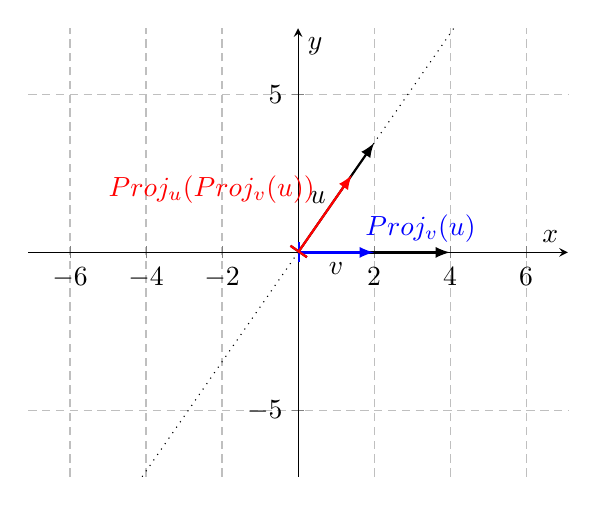
\begin{tikzpicture}[>=latex]
    \begin{axis}[
axis lines=middle,
grid,
grid style={densely dashed},
xlabel=\(x\), ylabel=\(y\),
xmin=-7.1, xmax=7.1,
ymin=-7.1, ymax=7.1
                ]
    \addplot [dotted, black]{1.732*x};
    \addplot [|->, thick,  black] coordinates {(0,0) (4,0)} node[near start, below] {$v$};
    \addplot [|->, thick,  black] coordinates {(0,0) (2,3.464)} node[midway, left] {$u$};
    \addplot [|->, thick,  blue] coordinates {(0,0) (2,0)} node[near end, above right] {$Proj_v(u)$};
    \addplot [|->, thick,  red] coordinates {(0,0) (1.414,2.449)} node[midway, above left] {$Proj_u(Proj_v(u))$};

    \end{axis}
\end{tikzpicture}
\end{center}

Como estão em direções diferentes, já é possível dizer que não são vetores iguais. $\blacksquare$

(b) VERDADEIRO. A soma de 2 vetores resulta em um vetor entre eles, seguindo um paralelogramo. Aplicando a reflexão R em v, obtem-se um vetor de mesmo módulo e mesmo ângulo em relação ao espelho. Pela simetria de $v + Rv$, daria um vetor na direção do espelho. $\blacksquare$

(c) FALSO. Definindo duas reflexões (Utilizando o fato que seus determinantes são -1) e fazendo sua composta:
\[R_1 = 
\begin{bmatrix}
1 & 3\\
0 & -1
\end{bmatrix}\]
\[R_2 =
\begin{bmatrix}
0 & 1\\
1 & 2
\end{bmatrix}\]
\[Q = R_1 R_2 = 
\begin{bmatrix}
3 & 7\\
-1 & -2
\end{bmatrix}\]
\[det(Q) = 1\]
Como o determinante de Q é 1, Q é uma rotação, não uma reflexão. $\blacksquare$
\end{document}
